\section{功能性需求}

本章节将阐述本系统的一系列功能需求。

\subsection{功能总览}

本系统拥有以下功能:
\begin{itemize}
    \item 用户登录
    \item 文件上传
    \item 文件下载
    \item 文件共享
    \item 图像文字识别
    \item 语音识别
\end{itemize}

\subsection{功能列表}

\subsubsection{用户登录}

\begin{figure}[H]
    \begin{center}
        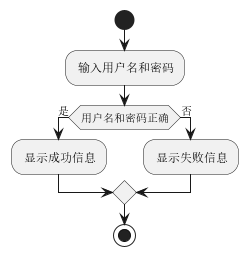
\includegraphics[scale=0.6]{examples/登录流程图.png}
        \caption{登录流程}
        \label{fig:login}
    \end{center}
\end{figure}

用户登录流程如图\ref{fig:login}所示,用户输入用户名和密码后判断是否正确,如果正确则成功登录。

\subsubsection{文件上传}

\begin{figure}[H]
    \begin{center}
        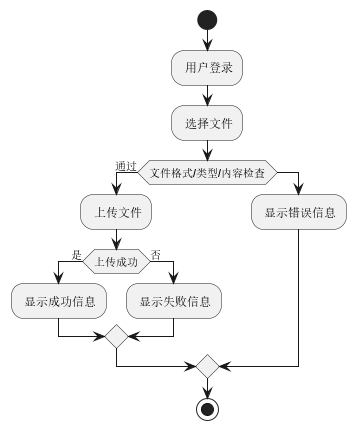
\includegraphics[scale=0.7]{examples/上传流程图.png}
        \caption{上传流程}
        \label{fig:upload}
    \end{center}
\end{figure}

文件上传流程如图\ref{fig:upload}所示,用户登录并选择文件后,对文件进行检查,检查成功后上传,如果成功,则展示成功信息。

\subsubsection{文件下载}

\begin{figure}[H]
    \begin{center}
        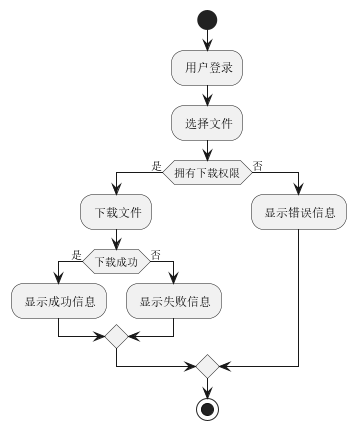
\includegraphics[scale=0.7]{examples/下载流程图.png}
        \caption{下载流程}
        \label{fig:download}
    \end{center}
\end{figure}

文件下载流程如图\ref{fig:download}所示,用户登录并选择文件后,检查下载权限,检查成功后下载,如果成功,则展示成功信息。

\subsubsection{文件共享}

\begin{figure}[H]
    \begin{center}
        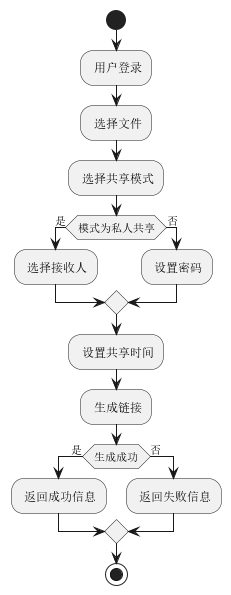
\includegraphics[scale=0.7]{examples/共享流程图.png}
        \caption{共享流程}
        \label{fig:share}
    \end{center}
\end{figure}

文件共享流程如图\ref{fig:share}所示,用户登录并选择文件后,选择共享模式:私人/公共,之后输入相关设置并生成共享链接。

\subsubsection{图像文字识别}

\begin{figure}[H]
    \begin{center}
        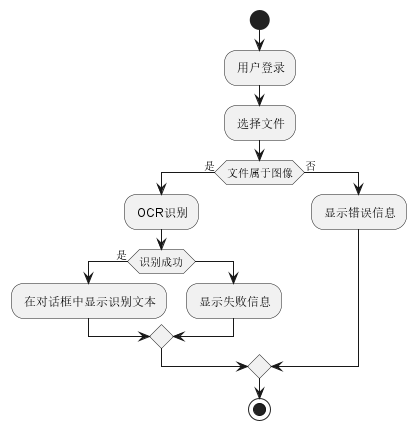
\includegraphics[scale=0.7]{examples/文字识别流程图.png}
        \caption{图像文字识别流程}
        \label{fig:textreg}
    \end{center}
\end{figure}

图像文字识别流程如图\ref{fig:textreg}所示,用户登录并选择文件后,判断文件是否属于图像,如果是,则调用OCR进行识别并展示。

\subsubsection{语音识别}

\begin{figure}[H]
    \begin{center}
        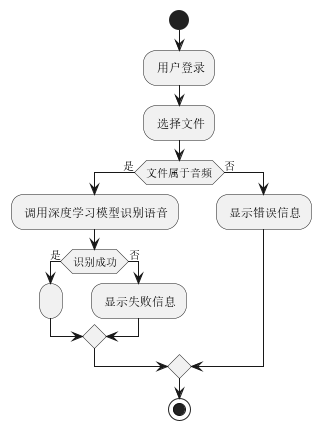
\includegraphics[scale=0.7]{examples/语音识别流程图.png}
        \caption{语音识别流程}
        \label{fig:audioreg}
    \end{center}
\end{figure}

语音识别流程如图\ref{fig:audioreg}所示,用户登录并选择文件后,判断文件是否属于音频,如果是,则调用深度学习模型进行识别并展示。

\subsection{接口描述}

\begin{table}[H]
    \centering
    \caption{接口描述}
    \label{table:api}
    {
        \begin{tabularx}{1.0\textwidth}{|p{1.5cm}|X|p{1.5cm}|X|X|}
            \hline
            功能 & URL & 请求方法 & 请求参数 & 响应结果 \\ 
            \hline
            用户登录 & /api/login & POST & 用户名、密码 & 状态码、消息 \\
            文件上传 & /api/upload & POST & 文件、用户ID、目标文件夹 & 状态码、消息 \\ 
            文件下载 & /api/download & GET & 文件ID & 文件 \\
            文件共享 & /api/share & GET & 文件ID、分享链接有效期 & 状态码、消息 \\
            文字识别 & /api/ocr & POST & 文件ID & 状态码、消息、识别结果 \\
            语音识别 & /api/speech & POST & 文件ID & 状态码、消息、识别结果 \\
            \hline
        \end{tabularx}
    }
\end{table}

主要的接口描述如表\ref{table:api}所示,基于HTTP协议设计,包含用户、文件等一系列操作。